\chaptertoc{}

\vspace{1em}

Until today, the \lya forest in quasar spectra has been the only 
tracer of large-scale structures producing measurements of 
baryon acoustic oscillations (BAO) at redshifts above 2. 
Given the higher redshifts and the smaller scales probed, 
the clustering of the forest also yielded competitive 
constrains on the sum of the mass of the neutrino species, 
when combining it with measurements of the cosmic microwave background (CMB)
anisotropies. Current and future spectroscopic surveys plan to observe  
denser samples of \lya forests to improve our understanding of the 
$z>2$ Universe.

In this chapter, I expose my contributions to the study of
dark energy through \lya forest observations. 
Section~\ref{forests:intro} introduce the main concepts used in 
this chapter. 
Section~\ref{forests:bao} focus on the BAO measurements from 
BOSS and eBOSS surveys for which I provided key contributions.
My thesis\footnote{\url{https://tel.archives-ouvertes.fr/tel-01389967}} 
was dedicated to this topic.
Section~\ref{forests:zerrors} and \ref{forests:lensing} 
present two projects carried out by my former PhD student  
Samantha Youles at the University of Portsmouth, UK, 
who graduated on the 18th of March 2022. 


\section{Forests as a tracer of the Universe's structures}
\label{forests:intro}

The \lya forest is the name for a series of absorption lines observed in quasar
spectra caused by the presence of neutral hydrogen along the line of 
sight between us and the quasars. 
Figure \textbf{XX} shows an example of a optical quasar spectrum with its \lya forest.
These lines are seen bluewards of the \lya emission peak of the quasar,
which lies at the quasar rest-frame wavelength $\lambda_\mathrm{rest}=1216~\angstrom$.
The absorption is not limited to the first transition; bluewards of the 
Ly$\beta$ peak ($\lambda_\mathrm{rest} = 1025~\angstrom$) we also observe 
Ly$\beta$ absorption lines on top of the \lya ones, and similarly for all
Lyman series until the Lyman break at 912~$\angstrom$.

The advatage of the forests is that it provides a tomographic 
view of the matter distribution along the line of sight of the quasar. 
This is because, as the light propagates outwards of the quasar, the 
Universe expands, causing the whole spectrum to be redshifted. 
When the redshifted spectrum hits a hydrogen atom, the light being
absorbed at the \lya transition in the \emph{atom} rest-frame 
is no longer at the \lya wavelength in the \emph{quasar} rest-frame:
it a bluer wavelength. If a given quasar sits at a redshift $z_q$ and 
a given intervening atom sits at a redshift $z_a < z_q$, the \lya photon being absorbed
by the atom corresponds to a photon at $\lambda_\mathrm{rest}= 1216(1+z_a)/(1+z_q)~\angstrom$
in the quasar rest-frame. In our frame, the observed wavelength of the 
atom absorption, or equivalently of its \lya line, is 
$\lambda_\mathrm{obs}= 1216(1+z_a)~\angstrom$. Note the 
observed wavelength does not depend on the quasar redshift.
We only need the quasar redshift to identify where the \lya forest is 
in the observed spectrum, such that we can assign each observed wavelength
to a quasar rest-frame wavelength. 
The result is that a single forest of lines maps the neutral
hydrogen density accros a large range in redshifts. One single
quasar spectrum can yield a map of the large-scale distribution 
of matter along its line of sight over up to several hundreds of 
megaparsecs (Mpc). 

How much neutral hydrogen is needed to create a forest of \lya 
absorption lines? Not a lot as it turns out. Given the 
high cross-section of the \lya resonance, very low densities of neutral 
hydrogen are sufficient to create a line. 
At redshifts $2 < z < 4$ where \lya forests are observed in the optical, 
typical densities found in the intergalactic medium (IGM), $n_\mathrm{HI} \sim 10^{XXX}~\si{\cm}^{-3}$,
are enough to absorb a significant fraction of the photons. 
Denser regions completely absorb the light and create saturated lines (zero flux). 
This is the case of the so-called \emph{high-column density systems} (HCDs), 
which are often associated with galaxies or proto-galaxies. The extreme cases 
can be observed with high-resolution spectrocopy, where we can also observe a non-saturated
\emph{deuterium} absorption from which we derive constraints on big-bang nucleosynthesis (BBN, 
see section~\ref{intro:probes:bbn}). 

The \lya forest, and therefore the amounts of neutral hydrogen in the IGM, 
is tighly connected with the process of reionisation of the Universe. 
As more stars and quasars form, more ultraviolet light is produced, 
progressively ionising the neutral hydrogen. On top of that, the Universe
continuously expands, diluting it. 
Thus, the average absorption of forests decreases with time, or increases with redshift.
At redshifts above 6, most of the light bluewards of the \lya emission is absorbed, 
while at redshifts below 1, the \lya absorption is minimal. 
Forests from $z_q>6$ quasars are used to put constraints on reionisation (ref?). 

The \lya forest and its connection with the large-scale structures have been studied 
theoretically since works by \cite{gunnDensityNeutralHydrogen1965}. Most of recent 
advances are thanks to numerical simulations. In order to simulate forests, 
a full hydrodynamic n-body simulations are required, including all the 
complex baryonic physics. \textbf{Add more refs. }
On large scales, it has been shown that the forest can be considered as 
linear tracer of the underlying matter field 
\cite{mcdonaldObservedProbabilityDistribution2000, mcdonaldMeasurementCosmologicalGeometry2003, 
mcdonaldLinearTheoryPower2005}. On smaller scales, the gas physics is more 
complex to model given the effects of pressure and thermal velocities. 
Feedback from supernovae explosions, AGN or star forming galaxies also play 
an important role to model the small-scale clustering (\cite{chabanierImpactAGNFeedback2020}). 
The small scales are 
interesting due to their potential to constrain neutrino masses for instance. 


The first measurements of clustering using the \lya forests 
were based solely on the two-point statistics along the same 
line of sight (\cite{croftPowerSpectrumMass1999, mcdonaldLyAlphaForest2006}). 
Given the good wavelength sampling of a forest, 
limited by the resolution of our spectrographs, the small scales 
are easily accessible in the radial/wavelength direction. 
This type of measurement is still 
performed today and allow us to obtain tight upper limits on 
the total mass of neutrino species (\cite{palanque-delabrouilleHintsNeutrinoBounds2020}), 
when combined with measurements of the cosmic microwave background. 

It is only with the Baryon Oscillation Spectroscopic Survey (BOSS) from SDSS-III 
that we could study the clustering of \lya forests in three dimensions. 
Thanks to the density of quasars observed by BOSS, of about 15~deg$^{-2}$, 
it was possible for the first time to estimate correlations using absorption 
from neighboring lines of sight. Also thanks to the large area of sky covered by 
BOSS, the first measurement of baryon acoustic oscillations (BAO) using forests was achieved 
\cite{buscaBaryonAcousticOscillations2013, slosarMeasurementBaryonAcoustic2013, kirkbyFittingMethodsBaryon2013}.

Quasars also trace the matter field. While their density is not homogenous enough across the sky 
to measure clustering using these quasars alone, they can be cross-correlated with 
the forests. The cross-correlation between quasars and \lya forests is interesting 
because it is mostly independent of the \lya forest auto-correlation. 
This is mainly because the quasar sample has a low density (shot-noise dominated).
The first measurement of BAO in the quasar-forest cross-correlation was also possible with 
BOSS (\cite{font-riberaQuasarLymanAlphaForest2014}). The BAO constraints from 
the auto and cross correlations could be combined assuming that these two are independent. 

Since the first measurements of BAO using forests, the BOSS and eBOSS collaborations 
published BAO constraints with increasingly larger samples and improved analysis.
They are associated with the official SDSS Data Releases (DR):
\begin{itemize}
 \item DR9: First measurement of large-scale \lya correlations without BAO (\cite{slosarLymanAlphaForest2011}); 
 \item DR9: First detection of BAO in the \lya auto-correlation 
            (\cite{buscaBaryonAcousticOscillations2013, slosarMeasurementBaryonAcoustic2013, kirkbyFittingMethodsBaryon2013});
 \item DR11: First detection of BAO in the quasar-\lya cross-correlation (\cite{font-riberaQuasarLymanAlphaForest2014}), 
             updated auto-correlation measurement (\cite{delubacBaryonAcousticOscillations2015});
 \item DR12: Final BOSS auto-correlation (\cite{bautistaMeasurementBaryonAcoustic2017}) 
             and cross-correlation measurements (\cite{dumasdesbourbouxBaryonAcousticOscillations2017});
 \item DR14: Updated measurements with eBOSS data (\cite{desainteagatheBaryonAcousticOscillations2019, blomqvistBaryonAcousticOscillations2019});
 \item DR16: Final \lya BAO measurements of SDSS (\cite{dumasdesbourbouxhelionCompletedSDSSIVExtended2020}).
\end{itemize}

\section{Baryon acoustic oscillations in the forests}
\label{forests:bao}

In this section I detail the methodology I used in my past work 
to measure BAO with a set of \lya forests, highlighting my 
personal contributions. I consider the case of SDSS forests, 
which are observed in the optical domain with low-resolution spectroscopy.
Forest have a rather low signal-to-noise ratio on average, 
so the methods are fit to this type of data. 
Similar methods are employed in the measurement of the line-of-sight
(or one-dimensionnal) power-spectrum, but we focus on BAO here. 

The main steps of the BAO analysis with \lya forests are:
\begin{itemize}
    \item estimate of the transmission field and their associated weights;
    \item estimate of the two-point correlation functions, including the cross-correlation with quasars;
    \item estimate of correction matrices due to distortions of continuum fitting and metals; 
    \item fit of the BAO model over measured correlations.
\end{itemize}

\subsection{Transmission field}
\label{forests:bao:transmission}

As described in section~\ref{forests:intro}, the amount of absorbed 
flux at a given wavelength (redshift) is related to the density 
of neutral hydrogen and therefore is a tracer of structures.  

The main observable used to compute correlations is the so-called
\emph{transmission} $F$, defined as 
\begin{equation}
    F(\hat{n}, \lambda) = f(\hat{n}, \lambda)/C(\hat{n}, \lambda) = \exp{-\tau(\hat{n}, \lambda)}
    \label{eq:transmission}
\end{equation} 
where 
$f(\hat{n}, \lambda)$ is the observed flux and 
$C(\hat{n}, \lambda)$ is the unabsorbed/original flux level, 
for a quasar line-of-sight at angular position $\hat{n}$ 
and observer-frame wavelength $\lambda$, which can be linked to the
absorber redshift $z = \lambda/\lambda_\alpha - 1$ if the absorption is 
due to \lya. We can also express the transmission as a function of the 
optical depth $\tau$ as in the right-hand side of Eq.~\ref{eq:transmission}.

The challenge is to estimate transmissions from the observed fluxes of a set of quasar
spectra, particularly given that our data is low-resolution and relatively noisy.
This makes it hard to ``see'' the unabsorbed flux level $C$, also known as the 
\emph{continuum} level, requiring automated methods. Several past attemps to achive this 
used either principal-component analysis techniques 
(\cite{leeMeanfluxregulatedPrincipalComponent2012}) where the templates were built from 
high-resolution and high signal-to-noise data; or maximum likelihood methods accounting
for the non-Gaussian nature of the probability density function of $F$ 
(\cite{buscaBaryonAcousticOscillations2013}). 
During my PhD, I particularly tried to merge these 
last two methods into a single one, without success. 
Those methods, while more sophisticated and flexible in their modelling of $C$, 
they suffer from the additional noise added to the estimated transmission 
due to noisier estimates of $C$. The simplest method will prevail in the latest
analyses, which consists in averaging forests in their rest-frame to obtain a
single average shape for $C$, or \emph{mean continuum} $\bar{C}$. 
This shape is then fitted to each individual forest with a linear tilt in $\log \lambda$,
i.e., $C(\hat{n}, \lambda) \equiv \bar{C}(\lambda) [ a_0(\hat{n}) + a_1(\hat{n})\log \lambda]$,
where $a_0$ and $a_1$ are fitted coefficients per quasar. 

Once the continnum level $C$ is estimated for each forest, one can compute 
the transmission $F$ and their \emph{fluctuations} $\delta_F$ around the mean,
defined as 
\begin{equation}
\delta_F(\hat{n}, \lambda) = \frac{F(\hat{n}, \lambda)}{\langle F \rangle} - 1
\label{eq:delta_transmission}
\end{equation}
where $\langle F \rangle$ is the ensemble-averaged transmission of the Universe. 

The $\langle F \rangle$ is actually an evolving function of time (or redshift or observed-frame 
wavelength) and it is important to take this evolution into account when computing 
$\delta_F$. 
Several measurements of this quantity exist 
(\cite{faucher-giguereDirectPrecisionMeasurement2008,
parisPrincipalComponentAnalysis2011,
beckerRefinedMeasurementMean2013,
kambleMeasurementsEffectiveOptical2020}), thought the latest BAO measurements do not 
use them directly to compute $\delta_F$. One could in principle use the forests themselves
to estimate $\langle F \rangle$, by stacking forests in their observer-frame 
(by contrast with the mean continuum that is a stack in the quasar rest-frame), 
though this requires a good estimate of $C$. 
If one express $\delta_F$ as a function of 
the observed flux $f$, the continuum $C$ and the average transmission $\langle F \rangle$,
one sees that there are degeneracies. 
The latest BAO analyses therefore fits a linear function 
that models the product $C \langle F \rangle$ simultaneously. 

All methods to estimate the transmission fluctuations also suffer from the fact 
that they use information the forests themselves to estimate $C$ or $C \langle F \rangle$.
This creates spurious correlations between a given pixel in a given forest and a neighboring 
pixel in the same forest. As I will discuss in section~\ref{forests:bao:matrices},
spurious correlations are also introduced between pixels in different lines-of-sight, 
distorting the correlation function. We name this effect the \emph{distortion
by continuum fitting}; it needs to be correctly modelled when fitting the 
correlation function.

Typical ranges chosen to define the \lya forest and extract the transmission field
are between 1040 and $1200~\angstrom$ in the quasar rest-frame. Recent analyses also 
consider the Ly$\beta$ forest region, between 920 and 1020~\angstrom, 
where both \lya and Ly$\beta$ absorption are present. The absorption in this region 
can be assigned a redshift that depends on the choice of $\lambda_\mathrm{rest}$, 
that can be either \lya$ = 1216~\angstrom$  or Ly$\beta = 1025$~\angstrom. 
These rest-frame wavelengths are separated enough such that both can be used 
in clustering measurements without much contamination at separations below 200\hmpc.

Uncertainties of the transmission fluctuations are also estimated from the data 
themselves. Typically two major components are taken into account when defining 
uncertainties: instrumental noise and the instrinsic variance of absorbers.
The former is essentially the output of the data reduction pipeline, described 
in Chapter~\ref{chap:spectro}, corrected with some normalisation factor. 
The latter is estimated from the variance of $\delta_F$ observed in the data. 
The intrinsic variance of $\delta_F$ is an increasing function of redshift, 
while the instrumental noise is typically decreasing with observer-frame wavelength, 
since forest mostly lie at the blue end of the spectrographs. 
The inverse of the final pixel uncertainty squared is used as a weight in the estimates of 
the correlation function.  

Word on DLAs ? 

Word on calibration residuals and my work to find/fix the problem ? 

\subsection{Two-point correlation functions}
\label{forests:bao:correlations}

Once the transmission fluctuations $\delta_F$ and their weights $w$ are estimated
for all pixels of all forests, we compute their auto-correlation function and 
their cross-correlation with quasars (or any other point tracer) in three dimensions, 
as a function of comoving radial and transverse separations. 

The first step is to convert redshifts to comoving distances using a fiducial cosmology. 
With angular positions and distances, we can obtain the separation $\vec{r} = (\rperp, \rpara)$
between two tracers, where $\rperp$ is the component orthogonal to the line-of-sight and 
$\rpara$ is the component along the line-of-sight. 

The correlations are estimated in bins of separation. We consider usually bins of 4\hmpc\ 
from 0 to 200\hmpc in both radial and transverse directions. For the cross-correlation 
with quasars, the radial separation can be negative, meaning that the absorber is closer 
than the quasar from us. Let $A$ be the index of a separation bin, the auto-correlation is 
defined as 
\begin{equation}
\xi^\mathrm{auto}_A = \frac{\sum_{i, j ~ \mathrm{if} ~ \vec{r}_{ij} \in A} w_i w_j \delta_{F, i} \delta_{F, j}}{\sum_{i, j ~ \mathrm{if} ~ \vec{r}_{ij} \in A} w_i w_j}
\label{eq:autocorrelation} 
\end{equation}
where the indexes $i, j$ denote a given pixel in the forest. The sum is over all pairs of 
absorbers for which the separation $\vec{r}_{ij} = \vec{r}_i - \vec{r}_j$ falls inside bin $A$. 

The cross-correlation of absorbers with quasars is estimated with the following estimator: 
\begin{equation}
    \xi^\mathrm{cross}_A = \frac{\sum_{i, j ~ \mathrm{if} ~ \vec{r}_{ij} \in A} w_i w_j \delta_{F, i}}{\sum_{i, j ~ \mathrm{if} ~ \vec{r}_{ij} \in A} w_i w_j},
    \label{eq:crosscorrelation} 
\end{equation}
which is very similar to the auto-correlation one in Eq.~\ref{eq:autocorrelation}.
The index $i$ runs over absorbers while $j$ runs over quasars, but there is no $\delta_{F,j}$ term. 
This estimator is valid under a few assumptions: sparcity of quasars, weak cross-correlation 
and weak auto-correlation. These assumptions are discussed in detail in the appendix B of
\cite{font-riberaLargescaleCrosscorrelationDamped2012}. 

The covariance matrix is estimated using sub-samples of the full survey. Under the 
assumption that each sub-sample $s$ is independent, the estimator of the covariance
between $\xi_A$ and $\xi_B$ is
\begin{equation}
C_{AB} = \frac{1}{W_A W_B} \sum_{s} W_A^s W_B^s [ \xi^s_A \xi^s_B - \xi_A \xi_B],
\label{eq:covariance-subsampling}
\end{equation}
where $W_A^s$ is the total weight in bin $A$ of sub-sample $s$ and $W_A \equiv \sum_s W_A^s$. 
This estimator has been tested with 100 realisations of synthetic datasets (mocks) and 
it shows to be robust at the current precision level. 

The data vector contains around 50x50 bins, making the covariance too large (2500x2500)
for the usual number of available sub-samples ($\sim 1000$). To avoid the matrix to be 
singular, we apply a smoothing to it. The smoothing procedure considers that the 
correlation coefficients, defined as $\rho_{AB} = C_{AB}/\sqrt{C_{AA} C_{BB}}$, 
are only a function of $\Delta \rperp \equiv \rperp_B - \rperp_A$ and 
$\Delta \rpara \equiv \rpara_B - \rpara_A$. By averaging all correlation coefficients
with the same $(\Delta \rperp, \Delta \rpara)$, we obtain a 50x50 matrix which is now 
positive definite. The new covariance matrix is constructed by taking these averaged 
coefficients and multiplying them by the variances. This method is used to estimate 
covariance matrices for both auto and cross correlation functions, but also for the 
cross-covariance between $\xi^\mathrm{auto}_A$ and $\xi^\mathrm{cross}_B$, used in 
joint fits (see section~\ref{forests:bao:model}).



\subsection{Correction matrices}
\label{forests:bao:matrices}

There are two important effects to be taken into account when modelling 
the \lya correlation functions: the distortion by the continuum fitting, discussed 
in section~\ref{forests:bao:transmission}, and the contamination by metal 
absorption. The most recent analyses use matrices to convolve a binned 
cosmological model and obtain the final template to be compared to 
the measured binned correlations. We describe both corrections below. 

The distortion matrix is built under the assumption that the ``mistake''
we make when fitting the continuum $C$ is also a linear function 
of $\log \lambda$. We therefore remove completely the components of $\delta_F(\lambda)$
that are proportional to a constant plus a slope. This procedure removes
not only the potential mistake we made, 
but also the cosmological signal proportional to a constant plus a slope,
though it is ok since these components should not contain much BAO information.
This removal of a linear component of $\delta_F$ is referred to as 
\emph{projection}\footnote{This is equivalent to the removal of modes 
contaminated by photometric systematics in galaxy clustering, as studied 
in \cite{paviotAngularSystematicsfreeCosmological2022}.}.
Thanks to the linearity of the problem, the model for the correlation function of 
the projected $\delta_F$ field can be written as a linear function of the 
true cosmological correlation function. For the case of a binned correlation function, 
this relation can be written with the help of a matrix, the \emph{distortion matrix}.
The distortion matrix was first introduced in \cite{bautistaMeasurementBaryonAcoustic2017}
for the BAO analysis of DR12 forests, where we showed that the distortion matrix 
was correctly describing the clustering of mock forests after continuum fitting. 

The contamination due to \emph{metal}\footnote{The term \emph{metal} is used in 
astronomy for elements heavier than helium.} 
absorption is mainly due to four transitions of silicon atoms for which their 
rest-frame wavelength is close to the \lya transition. When computing the 
auto-correlation of forests, metal absorption creates confusion because 
it is interpreted as a distinct \lya absorber when in fact it is the same. 
For example, the \textsc{SiIII} absorption happens at 
$\lambda_\mathrm{rest} = 1207~\angstrom$, close to \lya for which $\lambda_\mathrm{rest} = 1216~\angstrom$. 
In comoving coordinates, assuming a standard fiducial cosmology, this corresponds
to $\Delta \rpara \approx 21$\hmpc 
at $z \sim 2.3$. At these radial separations and when $\rperp \sim 0$, we see a 
spike in the correlation function. This peak is not due to \lya absorption 
separated by 21\hmpc but it is the cross-correlation between \lya and \textsc{SiIII}
absorption at near \emph{zero} separation. It is the same region in the 
Universe absorbing both in \lya and in \textsc{SiIII}, though the latter 
has a smaller amplitude. This happens for all metals with rest-frame 
wavelenghts close to \lya. For instance, one of the \textsc{SiII} transitions 
creates a spike at 111\hmpc, right at the BAO peak. 
Since \cite{delubacBaryonAcousticOscillations2015}, I worked on carefully 
adding metal absorption to mock forests in order to quantify their impact on 
BAO constraints. In \cite{bautistaMeasurementBaryonAcoustic2017}, we introduced 
a model for the \lya-metal cross-correlation to be fitted altogether with the 
BAO model. Similarly to the distortion modelling, the \lya-metal correlations 
can be described as a matrix times the \lya-\lya correlation function. 
This matrix is referred to as the \emph{metal matrix}. The amplitude of 
\lya-metal correlations is a free parameter in the BAO fits. 
We found that marginalising over these amplitudes makes BAO constraints 
slighly larger, though more conservative and robust.   

\subsection{The model}
\label{forests:bao:model}

The model used to fit for the BAO scale on the measured correlation functions 
is based on a linear matter power spectrum with some empirical terms 
that account for redshift-space distortions, non-linear clustering, 
high column density systems and binning effects. The model is constructed in 
Fourier space and it is Fourier transformed to obtain $\xi(\rperp, \rpara)$. 
The latest version of the model is described in \cite{dumasdesbourbouxhelionCompletedSDSSIVExtended2020}
and I shortly present it in this section. 

The model can be written, in Fourier space, as 
\begin{equation}
    P^\mathrm{model}(\vec{k}) = b_i b_j 
        \left(1+\beta_i \mu^2_k\right) \left(1+\beta_j \mu^2_k\right) 
        P_\mathrm{ QL}(\vec{k}) F_\mathrm{NL}(\vec{k})G_\mathrm{ bin}(\vec{k}), 
    \label{eq:power_spectrum}
\end{equation}
where $\vec{k}$ is the wavevector, with modulus $k$ and $\mu_k = k_\parallel/k$;
$b_i$ and $\beta_i$ are the linear bias and redshift-space distortions parameters, respectively,
and $i$ is a index referring to absorbers or quasars; 
$G_\mathrm{ bin}$ accounts for the binning of the correlation function, 
$F_\mathrm{NL}$ is a empirical term that accounts for the non-linear effects on small scales, 
and $ P_\mathrm{ QL}$ is the linear matter power spectrum with a empirical anisotropic 
damping applied to the BAO peak component. 
The linear matter power spectrum is computed from a Boltzmann solver code, 
such as \textsc{camb} (\cite{lewisEfficientComputationCosmic2000}). 

The non-linear term $F_\mathrm{NL}$ is only included for the quasar-\lya 
cross-correlation and accounts for the effect of Fingers-of-God on small-scales as well as 
an eventual contribution from uncertainties of redshift estimates,
which can be relatively large for quasars ($\sim 500$\kms). 
This term can be modelled as a Gaussian or as a Lorentzian, as a function of a 
velocity dispersion parameter $\sigma_v$ (in units of \kms).
The impact of redshift errors was studied in detail in 
\cite{youlesEffectQuasarRedshift2022} and it is also described in 
section~\ref{forests:zerrors}.

The effect of high-column density systems, if indentified and modelled 
when fitting the continuum, is negligible. For the HCDs that are 
not identified, the extended absorption (called ``wings'') causes 
$k_\parallel$-dependent broadening of the clustering 
(\cite{font-riberaEffectHighColumn2012,
rogersCorrelationsThreedimensionalLymanalpha2018}). 
This effect is modelled through effective biases $b_i^\mathrm{eff}$ 
and RSD parameters $\beta_i^\mathrm{eff}$ that depend on the 
biases of the \lya\ forest and those from HCDs, plus a function 
that depends on the distribution of column densities of the unidentified 
HCDs. 

The metal correlations are accounted as additive terms to the \lya 
correlations
\begin{equation}
\xi^\mathrm{model}_A =    \xi^{\mathrm{Ly}\alpha \times \mathrm{Ly}\alpha  }_A 
    + \sum_m \xi^{\mathrm{Ly}\alpha  \times m}_A
    + \sum_{m_1, m_2} \xi^{m_1 \times m_2}_A,
\end{equation}
where each $\xi^{m_1 \times m_2}$ can be written as a metal matrix 
$M_{A,B}$ times the $\xi^{\mathrm{Ly}\alpha \times \mathrm{Ly}\alpha  }_B$ 
as mentioned in section~\ref{forests:bao:matrices}. The metal matrix is 
defined as 
\begin{equation}
M_{A,B} = \frac{1}{W_A}  \sum_{(m,n)\in A, (m, n)\in B} w_m w_n, 
\end{equation}
where $(m, n)\in A$ refers to pixel separations computed assuming 
\lya\ absorption, while $(m, n)\in B$ refers to pixels separations  
computed assuming metal absorption. This formalism was introduced 
in \cite{blomqvistTriplyionizedCarbonForest2018}. 

Quasars emit UV photons which ionise their surroundings slightly 
more than the average intergalactic medium. This is known as the 
\emph{proximity effect} and it changes the average properties of 
\lya absorption and therefore its clustering. When considering 
forests around a given quasar but not to its own forest, we refer 
to it as the transverse proximity effect. This effect is accounted  
for in the quasar-\lya cross-correlation with the following parametric
form:
\begin{equation}
\xi^{TP} = \xi_0^{TP} \left( \frac{1 h^{-1} \mathrm{Mpc}}{r} \right)^2 \exp \left( - r /r_{UV} \right)
\end{equation}
where $r^2 = \rpara^2 + r^2_\perp$, $r_{UV} = 300$\hmpc is fixed and $\xi_0^{TP}$ 
is a fitted amplitude. 

The spectroscopic data reduction pipeline described in section~\ref{spectro:pipeline2d}
also introduces spurious correlations between spectra. 
For instance, sky-subtraction and flux calibration are two processes 
that induce correlation between two pixels at the same observed wavelength 
but in two distinct lines-of-sight, provided they are observed with the 
same spectrograph (set of 500 fibers). These correlations have been 
studied using quasar spectral regions deprovided of \lya absorption,
such as the MgII spectral region ($\lambda_\mathrm{rf} \in [2600, 2760]$\angstrom).
An empirical model for this effect is included: a Gaussian, function of $\rperp$, centered in $\rperp = 0$ 
but only when $\rpara = 0$. 
Due to the effect of distortion caused by continuum fitting, these spurious
correlations due to data reduction also propagate to pairs with $\rpara \neq 0$.  
The amplitude and characteristic length of this effect are two free parameters
in the fit of the \lya auto-correlation function.

The correlation function model accounts for the distortion 
matrix, as discussed in section~\ref{forests:bao:matrices}. 
The distorted correlations are written as
\begin{equation}
    \xi^\mathrm{ dist}_A = \sum_{A'} D_{AA'} \xi^\mathrm{ model}_{A'}.
    \label{eq:xi_distorted}
\end{equation}  

It is also possible to add arbitrary smooth functions of separation
in order to account for any unexplained correlations and improve the fit
to the data. These functions are used to marginalise over any potential 
information on BAO coming from the full-shape of the correlation functions, 
which is avoided. This is commonly done in galaxy clustering analysis 
as I will show in Chapter~\ref{chap:galaxies}.


\subsection{BAO constraints}
\label{forests:bao:constraints}

The last essential ingredient to be added to the model of correlations
are the Alcock-Paczynski (AP) parameters. 
Thanks to the observed baryon acoustic scale, which we know should be isotropic and 
have a comoving size of $r_d \sim 105$\hmpc, the AP parameters can be well 
constrained with the data. These AP parameters account for small differences between 
the assumed fiducial cosmology, used to convert redshifts into distances, 
and the measured cosmology extracted from the observed BAO peak position.

We commonly use two AP parameters, encoding radial and transverse dilation 
effects. They can be written as ratios of the observed $\Delta z_\mathrm{BAO}$
and $\Delta \theta_\mathrm{BAO}$ at a given effective redshift $\zeff$ 
from equations~\ref{eq:bao_radial} and \ref{eq:bao_angular}
of section~\ref{intro:probes:bao}, yielding
\begin{equation}  
    \apara(\zeff) = \frac{D_H(\zeff)}{D_H^\mathrm{fid}(\zeff)} \frac{r_d^\mathrm{fid} }{r_d}
    \label{eq:alpha_parallel}
\end{equation}
\begin{equation}  
    \aperp(\zeff) = \frac{D_M(\zeff)}{D_M^\mathrm{fid}(\zeff)} \frac{r_d^\mathrm{fid} }{r_d}
    \label{eq:alpha_perp}
\end{equation}
where $D_H$ and $D_M$ are respectively the Hubble and comoving angular diameter distances
(Eqs.~\ref{eq:hubble_distance} and \ref{eq:comoving_ang_diameter_distance}).

The AP parameters $\apara$ and $\aperp$ are used to scale separations when 
computing the correlation function model as
\begin{equation}
    \xi(r'_\perp, r'_\parallel)  = \xi(\aperp \rperp, \apara, \rpara),
\end{equation}
and they are let free when fitting correlations. 
The BAO constraints are defined by the posteriors of $\aperp$ and $\apara$, 
after marginalising over all other free parameters of the model. 


Figure~\ref{fig:baolya_dr16} shows the current BAO constraints from the 
SDSS DR16 sample of \lya forests (containing both \lya and \lyb absorption) 
and quasars (\cite{dumasdesbourbouxhelionCompletedSDSSIVExtended2020}). 
The marginalised constraints from the joint fit of 
auto and cross-correlations are 
\begin{eqnarray}
    D_H(z = 2.334)/r_d & = & 8.99^{+0.20}_{-0.19} \\ 
    D_M(z = 2.334)/r_d & = & 37.5^{+1.2}_{-1.1} \\
    \rho( D_H/r_d, D_M/r_d) & = & -0.45 
\end{eqnarray}
which represent a 2.2 per cent BAO measurement in the radial direction 
and a 3.2 per cent in the transverse direction. 


\begin{figure}[t]
\centering 
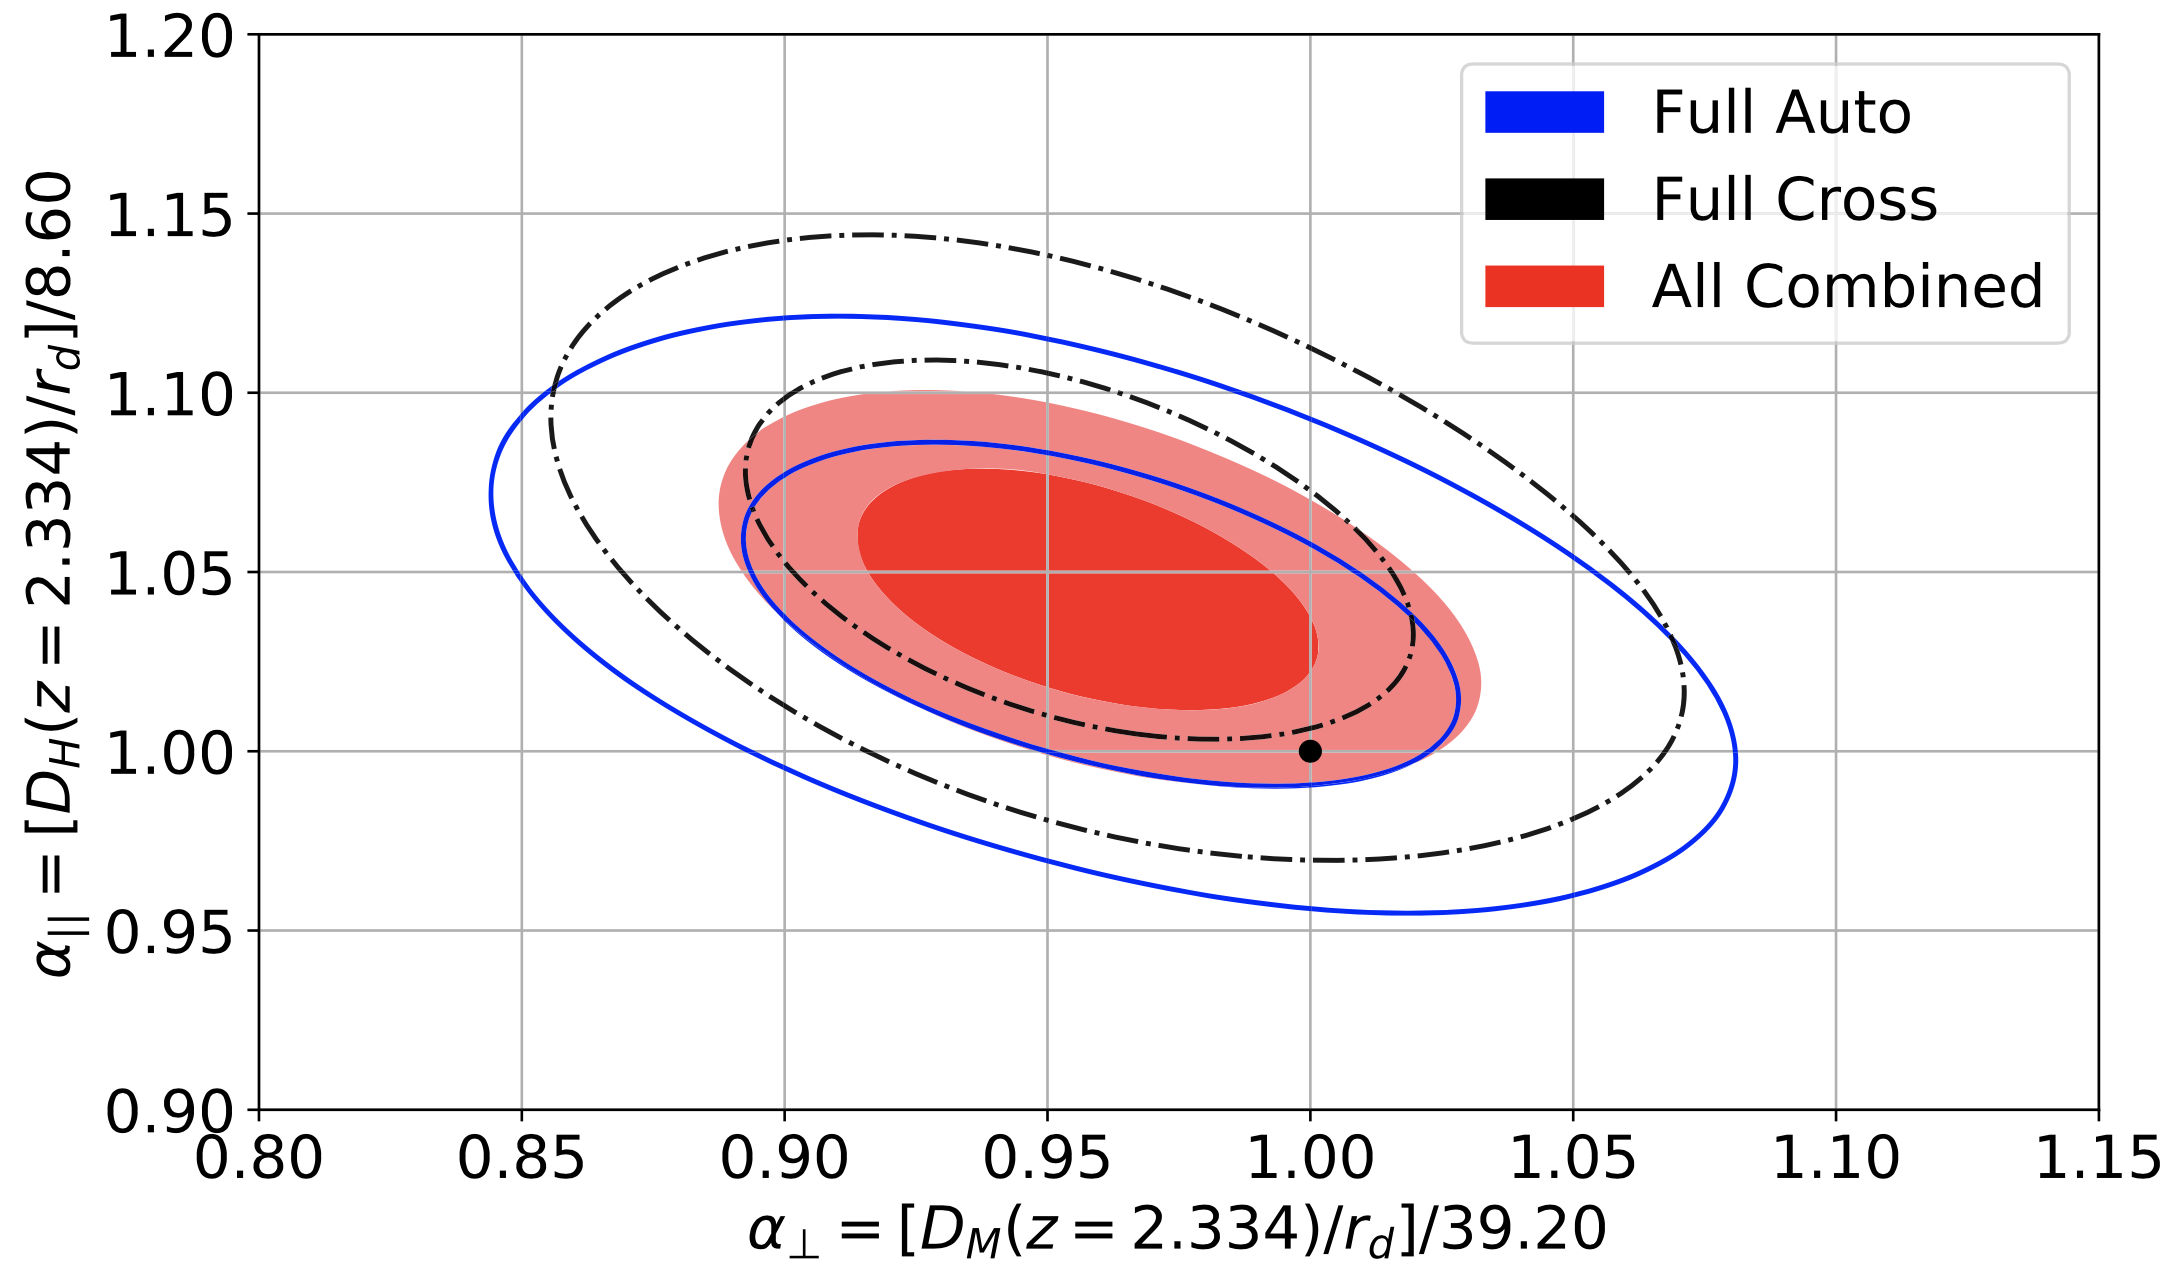
\includegraphics[width=0.6\textwidth]{fig/forests/baolya_dr16.png}
\caption{BAO constraints from the SDSS DR16 sample of \lya forests. 
The contours show the 68 and 95 per cent confidence levels for the 
Alcock-Paczynski parameters $\aperp$ and $\apara$ from the fits to 
the \lya-\lya auto-correlation (blue solid), 
the quasar-\lya cross-correlation (black, dash-dotted), and the  
joint fit of auto+cross (red shades).
Given the high level of shot-noise of the quasar sample, the 
covariance between constraints from the auto and cross correlation are found to be 
negligible.
Extracted Figure 12 from \cite{dumasdesbourbouxhelionCompletedSDSSIVExtended2020}.}
\label{fig:baolya_dr16}
\end{figure}




\section{Impact of redshift errors}
\label{forests:zerrors}

This section concerns work led by Samantha Youles, PhD candidate under 
my supervision at the University of Portsmouth between 2018 and 2022. 
The full details are presented in \cite{youlesEffectQuasarRedshift2022}. 

A key element in the BAO analysis using forests is the quasar redshifts, 
which can be challenging to measure precisely when compared to galaxy redshifts. 
Quasar spectra are basically composed of thermal continuous emission 
from their accretion disk around their supermassive
black holes in the centre of their host galaxies plus some broad emission lines. 
Typical quasar spectra from SDSS or DESI do not present detected narrow absorption or 
emission lines from the host galaxy itself, which would considerably improve the 
uncertainties on their redshifts. Previous studies using quasars as tracers for 
clustering (\cite{zarroukClusteringSDSSIVExtended2018, lykeSloanDigitalSky2020}) 
estimated that quasar redshift uncertainties range from 
100\kms at $z\sim 1$ to 400\kms at $z\sim 2$, while galaxies (LRGs or ELGs) have 
redshift uncertainties below $\sim 50$\kms. Of course, these uncertainties 
depend on the spectrograph and on which broad emission lines are visible
for a given quasar. 

In addition to statistical uncertainties in the determination of redshift, 
\cite{shenSloanDigitalSky2016} has shown that redshifts derived from 
broad emission lines of quasars have intrinsic scatter and systematic shifts
of the order of hundreds of \kms with respect to the host galaxy redshift. 
Current redshift fitting algorithms based on templates do not account for these shifts. 
While \cite{youlesEffectQuasarRedshift2022} studies the impact of scatter, 
we did not study in detail the impact of systematic shifts. 


The uncertainties in the redshift measurements smear the two-point statistics 
of the quasars over separations along the line-of-sight. The smearing directly 
impacts the BAO measurement, particularly reducing the signal-to-noise ratio 
of estimates of $\apara$ (see section~\ref{forests:bao:model}). 

Non-linearities induce large peculiar velocities on scales below a few Mpc
and are commonly modelled as a random scatter in the radial direction.
These non-linearities are known as \emph{fingers-of-God} (FoG) and they smear
the two-point statistics in a similar manner than redshift errors, though 
I will show the differences. 

In this section, these two types of extra scatter in quasar redshifts are parametrised by
\begin{itemize}
 \item $\sigma_{v, z}$ as the scatter induced by uncertainties in redshift determination, or redshift errors.
 \item $\sigma_\mathrm{v, FoG}$ as the scatter induced by non-linear motions on small scales, or Fingers-of-God.
\end{itemize}

Using DESI mock catalogues of the 5-year sample of \lya forests and quasars, 
we studied the impact of each of these types of extra scatter on the clustering and 
on BAO constraints. We discovered a new feature arising from redshift errors that 
modifies the shape of the two-point statistics in a non-trivial manner, 
though it does not impact BAO constraints expected with DESI. 




Figure~\ref{fig:zerrors_correlations} presents correlation functions, both 
for the quasar-\lya cross-correlation and for the \lya auto-correlation, 
in averages over $\mu_r \equiv \rpara/r$. There are three sets of mocks
\begin{itemize}
\item[1)] fiducial ones where $\sigma_\mathrm{v, FoG} = 150$\kms and $\sigma_{v, z} = 0$, 
\item[2)] mocks with $\sigma_\mathrm{v, FoG} = 500$\kms and $\sigma_{v, z} = 0$ and 
\item[3)] mocks with $\sigma_\mathrm{v, FoG} = 150$\kms and $\sigma_{v, z} = 500$\kms. 
\end{itemize}

\begin{figure}
    \centering 
    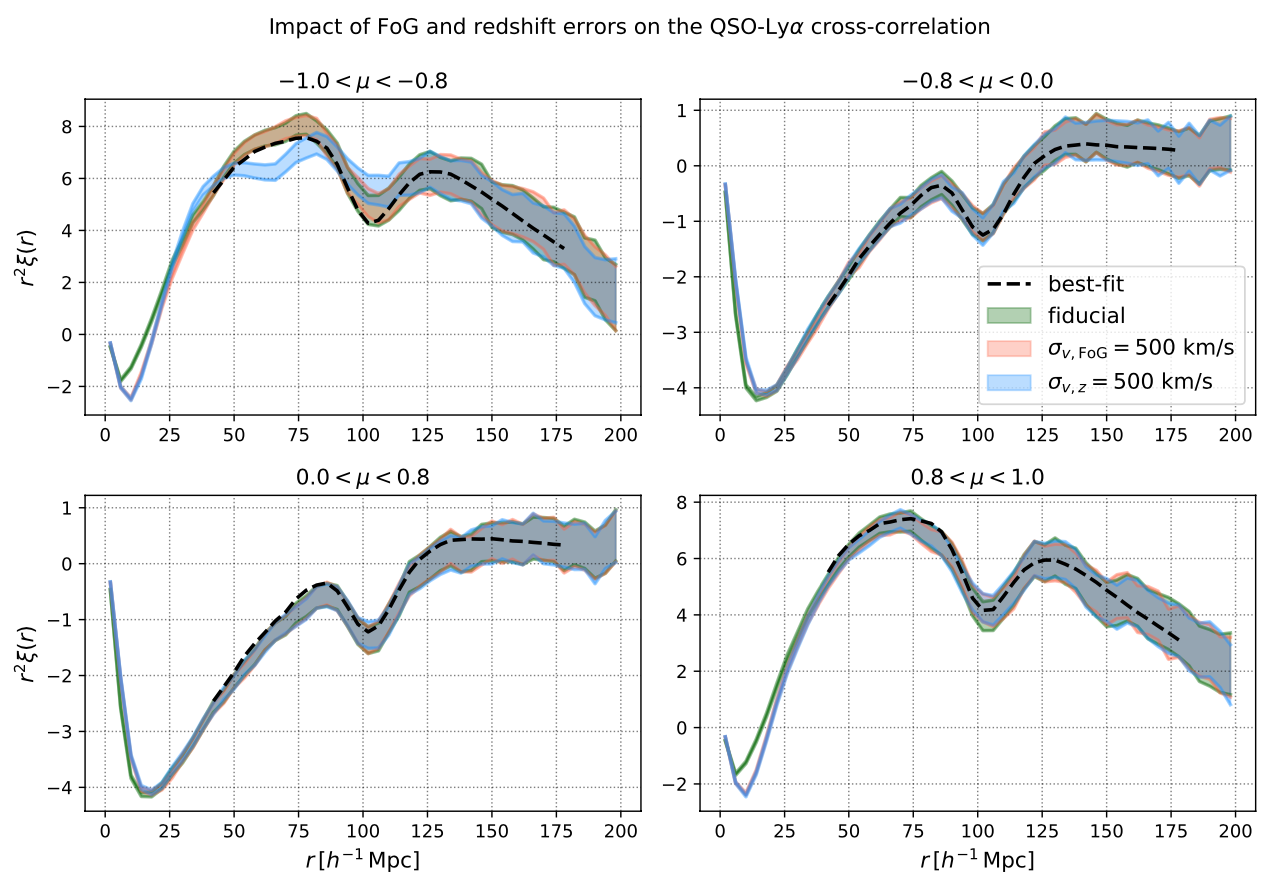
\includegraphics[width=\textwidth]{fig/forests/zerrors_cross.png}
    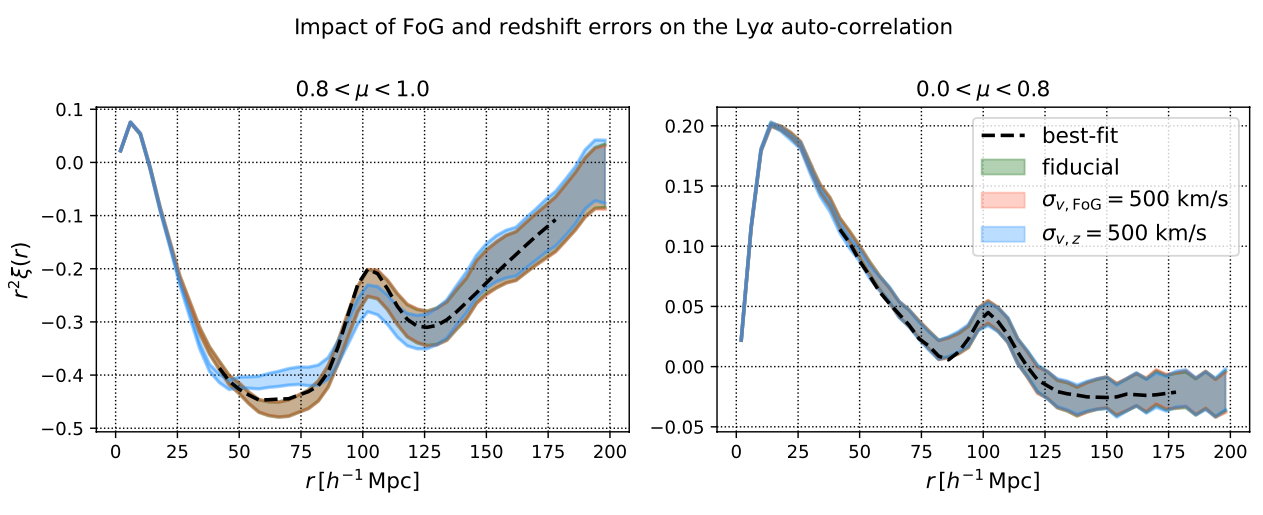
\includegraphics[width=\textwidth]{fig/forests/zerrors_auto.png}
    \caption{Wedges of the correlation functions versus comoving separation. 
    Top four panels show the QSOx\lya cross-correlation (top four panels) 
    while the bottom two panels show the \lya auto-correlation of forests. 
    These are estimated from DESI mock catalogues reproducing the full 5-year sample. 
    The green bands show the measurement from the standard mocks, 
    with a small value of $\sigma_\mathrm{v, FoG} = 150$\kms and no redshift errors; 
    the pink bands (indistinguishable from the green in the cross-correlation) 
    correspond to the mocks generated with an extreme value of 
    $\sigma_\mathrm{v, FoG} = 500$\kms; 
    the blue bands shows the results for mocks with large redshift errors of 
    $\sigma_\mathrm{v, z}= 500$\kms. 
    These measurements are computed from the average of 10 realisations of the 
    complete 5-year DESI survey, and the width of the bands corresponds to the 
    scatter between realisations. 
    Note that $\mu > 0$ ($\mu < 0$) corresponds to configurations where 
    the \lya  pixels are behind (in front of) the neighbouring quasar.
    }
    \label{fig:zerrors_correlations}
\end{figure}

Each set of mocks contains ten realisations, results are averaged for each set.
The colour bands show the scatter amongst realisations and are equivalent to the
noise expected for the 5-year sample. We can see that FoG (orange bands) do not 
have a significant impact except on the cross-correlation on small scales. 
However, redshift errors do create a new oscillatory feature both in the auto 
and cross-correlations at separations of 20-50\hmpc but only those along the 
line-of-sight. Using other mock catalogues with increasing values of 
$\sigma_{v, z}$ (not shown here) makes these features stronger. 
This work puts in evidence this effect for the first time. 

In \cite{youlesEffectQuasarRedshift2022}, we claim that the oscillatory
features appearing when adding redshift errors to quasars is due to 
two main factors: the smoothing of emission lines in the continua and 
the clustering of the quasars. These two factors \emph{combined} create this new 
effect. The smoothing of the mean continuum is illustrated in Figure~\ref{fig:zerrors_continua}
for increasingly large values of $\sigma_{v, z}$. These oscillatory features 
defined by the difference between true and estimated continua are imprinted 
on the clustering thanks to the fact that quasars themselves are clustered. 


\begin{figure}
%\begin{wrapfigure}{r}{5.5cm}
    \centering 
    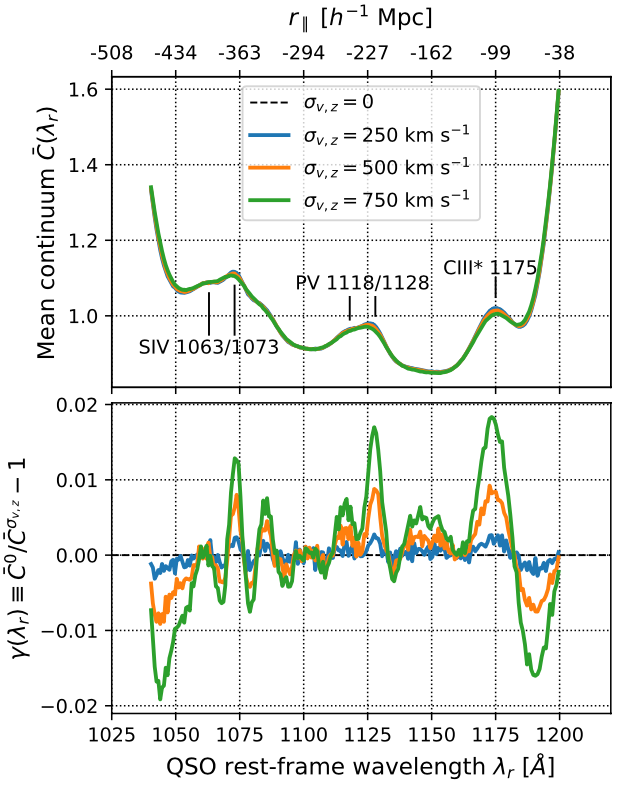
\includegraphics[width=0.5\textwidth]{fig/forests/zerros_impact_continua.png}
    \caption{Effect of redshift errors on the mean continuum. 
    The top panel shows the mean continua for no-forest mocks without errors, 
    and with increasingly large redshift errors: $\sigma_{v, z} = 0$, 250, 500 and 750\kms. 
    The positions of some of the strongest emission lines are annotated. 
    The lower panel shows the ratio between the continua with and without redshift errors. 
    The top axis on the top panel shows the radial separations between pixels and the quasar, 
    assuming that the quasar is at redshift $z_q = 2.3$.}
    \label{fig:zerrors_continua}
%\end{wrapfigure}
\end{figure}

We tested our hyphotesis by creating two special sets of mock catalogues, one 
where quasars are deprovided of forest absorption, and one where quasars are 
not clustered. With the first set of mocks, features are still present with the 
same amplitudes as the standard mocks. 
This points to the fact that the \lya forest and their correlations do not play 
a role in this effect. 
For the second set of mocks, the features disappear in the correlation functions, 
demonstrating that the quasar clustering is a key ingredient to explain the effect. 

While this model is satisfactory to explain the features in the cross-correlation, 
the auto-correlation seems to require an additional ingredient that we could not 
identify. We leave this investigation for future work. 

We performed BAO fits on all sets of mocks for different values of 
$\sigma_{v, z}$ and $\sigma_\mathrm{v, FoG}$. We employ the exact same model 
described in section~\ref{forests:bao:model}, though we did not include 
metals or high-column density systems. We do not attempt to model 
the effect of redshift errors when fitting for BAO. 
We see an increased value for the $\chi^2$ of the fits when increasing 
the value of $\sigma_{v, z}$, simply because these features are not modelled
properly. The inferred BAO parameters $\apara$ and $\aperp$ do not see 
significant shifts or trends versus $\sigma_{v, z}$ other than a slight increase 
in their uncertainties. 

We believe that for the final analysis of the 5-year DESI sample the impact 
of redshift errors has to be correctly modelled in order to reduce the 
uncertainites in BAO parameters or to extract cosmological information from  
the full-shape of the correlation function \cite{cuceuCosmologyBAO3D2021}.

\section{Weak-lensing of forests}
\label{forests:lensing}

This section also concerns work led by Samantha Youles, PhD candidate under 
my supervision at the University of Portsmouth between 2018 and 2022. 

\section{Voids in tomographic maps}
\label{forests:voids}

\cite{ravouxFirstMeasurementCorrelation2022}


